\documentclass[12pt, a4papre]{article}
\usepackage[catalan]{babel}
\usepackage[unicode]{hyperref}
\usepackage{amsmath}
\usepackage{amssymb}
\usepackage{amsthm}
\usepackage{xifthen}
\usepackage{siunitx}
\usepackage{xcolor}
\usepackage{float}
\usepackage[utf8]{inputenc}

\usepackage{listings}
\usepackage{setspace}
\usepackage{graphicx}
\usepackage{tikz,lipsum,lmodern}
\usepackage[most]{tcolorbox}
\usepackage{circuitikz}
\usepackage{indentfirst}
\usepackage{verbatimbox}
\definecolor{mygreen}{RGB}{28,172,0} % color values Red, Green, Blue
\definecolor{mylilas}{RGB}{170,55,241}
\usepackage{listings}
\lstdefinelanguage{vhdl}{
   morekeywords={
     library,use,all,entity,is,port,in,out,end,architecture,of,
     begin,and
   },
   morecomment=[l]--
}
\usepackage{xcolor}
\colorlet{keyword}{blue!100!black!80}
\colorlet{comment}{green!50!black!90}
\lstdefinestyle{vhdl}{
   language     = VHDL,
   basicstyle   = \ttfamily,
   keywordstyle = \color{keyword}\bfseries,
   commentstyle = \color{comment}
}

\graphicspath{ {./.} }


\newcommand{\norm}[1]{\lvert #1 \rvert}

\hypersetup{
    colorlinks = true,
    linkcolor = blue
}

\author{Daniel Vilardell}
\title{\textbf{Memoria Practica 2}}
\date{}

\begin{document}
	\maketitle
	
	\textbf{3.2 Dependència angular de les components del camp B}
	
	\textbf{a)}
	
	\begin{center}
		\begin{tabular}{ |c | c  c  c  c|}
			\hline
			$\theta$[º] & V[V]	& $B_r$[G] 	& $B_r$ de fons[G] & $B_r$ creada per iman[G] \\ \hline
			0 &-0.669 		 					& -66.9  				& 1.3		&   -68.2\\ 
			15 &-0.642						& -64.2				& 1.2		&   -65.4\\
			30 & -0.579						& -57.9				&1.4		&   -59.3\\
			45 &-0.457						& -45.7				& 1.54	&   -47.24\\
			60 &-0.294 						& -29.4				& 1.5		&   -30.9\\
			75 &-0.114 						& -11.4				& 1.5		&   -12.9\\
			90 &-0.075						& -7.5				& 1.6		&   -9.1\\
			\hline
		\end{tabular}
	\end{center}
	
	\textbf{b)}
	
	\begin{center}
		\begin{tabular}{ |c | c  c  c  c|}
			\hline
			$\theta$[º] & V[V]	& $B_{\theta}$[G] 	& $B_{\theta} $de fons[G] & $B_{\theta}$ creada per iman[G] \\ \hline
			0 &-0.047	 					& -4.7  				& 1.8		&   -6.5\\ 
			15 &0.037						& 3.7					& 1.9		&   2\\
			30 & 0.128					& 12.8				&1.8		&   11.0\\
			45 &0.244						& 24.4				& 1.7		&   22.7\\
			60 &0.347						& 34.7				& 1.5		&   33.2\\
			75 &0.372 					& 37.2				& 1.2		&   36\\
			90 &0.405						& 40.5				& 1.1		&   39.4\\
			\hline
		\end{tabular}
	\end{center}
	
	\textbf{c)}
	
	\begin{center}
		\begin{tabular}{ |c | c | c | c |}
			\hline
			$\theta$[º]  & $B_{\theta}$ creada per iman[G] & $B_r$ creada per iman[G]  \\ \hline
			0 		&   -6.5		&   -68.2\\ 
			15 		&   2			&-65.4\\
			30 		&   11.0		&-59.3\\
			45		&   22.7		&-47.2\\
			60 		& 33.2		&-30.9\\
			75 		&   36		&-12.9\\
			90		&  39.4		&-9.1\\
			\hline
		\end{tabular}
	\end{center}
	
	\begin{center}
		\begin{tabular}{ |c | c | c | c |}
			\hline
			$\theta$[º]  & $B_{\theta}$ creada per iman[G] normalitzat & $B_r$ creada per iman[G] normalitzat \\ \hline
			0 		&   0.09			&   1\\ 
			15 		&   -0.03			&0.95\\
			30 		&   -0.16			&0.86\\
			45		&   -0.33			&0.69\\
			60 		&  -0.49			&0.45\\
			75 		&   -0.52			&0.19\\
			90		&  -0.57			&0.13\\
			\hline
		\end{tabular}
	\end{center}
	
	Podem veure que el resultat experimental concorda amb el teoric ja que si ho grafiquem $B_{\theta}$, taronja, es mostra aproximadament com un cosinus de amplitud 1 mentres que $B_r$ es mostra com un sinus d'amplitud 0.5.
	\begin{figure}[H]
		\begin{center}
		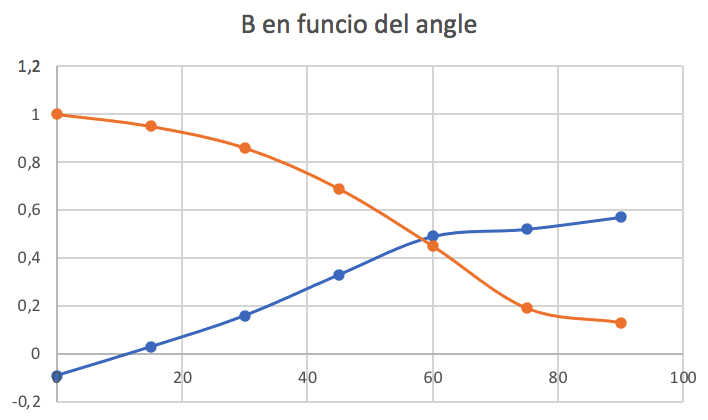
\includegraphics[width=130mm]{GraficaEM.png}
		\end{center}
	\end{figure}
	
\end{document}





